\begin{qBox}{1}
Implement the routines listed in \texttt{neural.h}, as was discussed in class. 
These, together with the lattice functions provided in the \texttt{Ising} package,
should enable you to create a functional Hopfield neural network.
After checking that your network functions in a manner similar to what was demonstrated in class, use your network to decode the mystery characters in the \texttt{final}
directory on the git repo.
There are seven distorted patterns (001.dat - 007.dat) in the \texttt{mystery}
subdirectory.
For each of these patterns: 

\begin{itemize}
    \item Load your network with the four patterns in \texttt{character\_groups} that 
        correspond to the numbered mystery pattern.
    \item Evolve the network.
    \item This is hopefully result in convergence to the correct, undistorted pattern.
        Your evolved pattern should match one of the four inputs exactly, giving a 
        Hamming distance of zero. Store or record the character you converge to.
\end{itemize}

String the seven decoded patterns together, in order. What's the mystery word?

\tcblower

The mystery word that I obtained was: PHYS352.
\baseSkip 

Although I was able to converge in on the correct pattern, the Hamming distance for 
"H" was not zero; rather, the Hamming distance for and "H" was \( 0.080 \) as shown below:

\begin{figure}[H]
    \centering
    \begin{minipage}{0.45\linewidth}
        \centering 
        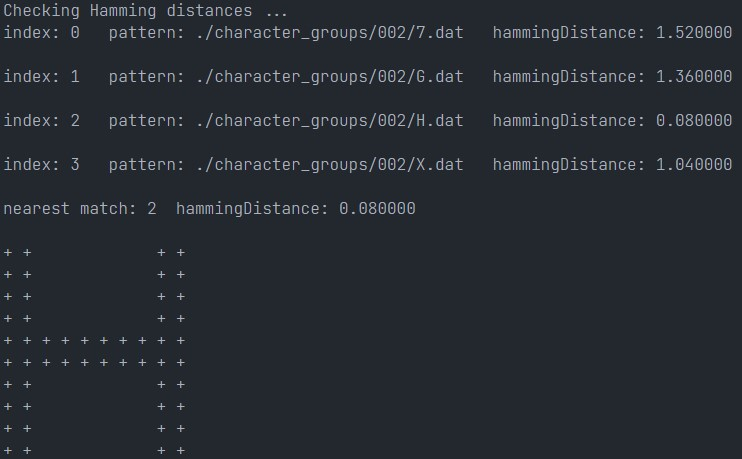
\includegraphics[ width = 0.95\linewidth ]{figures/H.jpg}
    \end{minipage}
    \begin{minipage}{0.45\linewidth}
        \centering 
        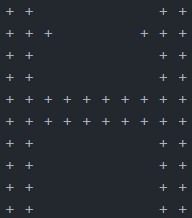
\includegraphics[ width = 0.5\linewidth ]{figures/H_Conserved.jpg}
    \end{minipage}
    \caption{The Hamming Distance for "H" and the measured converged character.}
\end{figure}

After running the program several, several times, I consistently kept getting this 
exact Hamming distance value. 
One possibility that I could think of for why I was seeing such values was that the 
converged character that I kept getting (as shown above) was another minimum. 
One possible fix to this issue (I think) would be to 
increase the temperature; doing so would increase the variability/scope so that we can land in the minimum that we want. 

\baseSkip

I have tried to implement this change, but saw varying results.
For example, when I increased the temperature slightly, I was indeed able to 
obtain Hamming distance values of \( 0 \) for "H" -- but at the expense of other 
characters to have a nonzero Hamming distance value.
The only other possibility is in how I implemented the code, but I currently do not see 
any issues with the implementation with respect to what the text and lectures suggest;
however, I could be (most likely) wrong here.
At the very least, we do see that the Hamming distance value for "H" is much smaller
than the other Hamming distance values within that group.

\baseSkip 

The entire output of the program can be seen in \texttt{output}.
\end{qBox}